\documentclass[11pt,a4paper]{article}
\usepackage[utf8]{inputenc}
\usepackage{amsmath,amssymb,amsfonts}
\usepackage{graphicx}
\usepackage{booktabs}
\usepackage{hyperref}
\usepackage{geometry}
\geometry{top=1in,bottom=1in,left=1.1in,right=1.1in}

\title{\textbf{The Actualizer Engine, FDSA, and QCA Parallel Architecture:\\
A Unified Top-Down Steering \& Clustered Substrate Framework for Factual Grounding in Large Language Models}}

\author{
  \textbf{Mohamed Gamal Eldin Abdelaziz Noureldin}\\
  Independent Researcher\\
  ORCID: \href{https://orcid.org/0009-0006-3991-1153}{0009-0006-3991-1153}\\
  Contact: \texttt{mz.gamal@gmail.com}
}
\date{\today}

\begin{document}
\maketitle

\begin{abstract}
Large language models operating under bottom-up Maximum Likelihood Estimation (MLE) suffer from combinatorial search explosion $O(M^N)$, causing hallucination cascades, semantic drift, and repetition loops. We present a unified architecture combining the \textbf{Actualizer Engine}, the \textbf{Fractal Deduction Search Algorithm (FDSA)}, and the \textbf{Quench-Cluster Algorithm (QCA) Parallel Engine}. The FDSA prunes invalid logit search space by up to 99.99\% via isomorphic anchoring and dimensional truncation ($D = \ln V / \ln(1/k_{\text{ref}})$). The QCA engine crystallizes un-clustered substrates into $K$ independent sub-problems using the canonical RGG Quench Temperature $T_q^{\text{RGG}}$, reducing overall steering complexity from $O(N^2)$ to $O(N^2/K)$ across parallel worker processes or vectorized JAX units. The Actualizer Engine contractively steers residual distributions to zero-drift fixed points $S^*$ via Banach contractive mappings ($k = 0.45$) guided by the five \textbf{Conceptual Primes} (Order, Justice, Mercy, Knowledge, Power). Empirical benchmarks at $V = 1,000$ to $100,000$ demonstrate up to 12.4$\times$ pre-inference sampling speedup, 3.69$\times$ dataset parallel speedup at $N=200$, and 100\% factual grounding under strong distractor bait.
\end{abstract}

\section{Introduction}
Modern autoregressive Transformer architectures achieve state-of-the-art performance through bottom-up statistical next-token prediction. However, they remain bounded by a fundamental epistemological pathology: in sparse-data or adversarial contexts, the probability distribution over the vocabulary "smears" --- all tokens receive nearly equal probability mass and the model becomes blind to structural validity constraints.

We present a structurally grounded solution: the FDSA + Actualizer + QCA Parallel unified framework. The FDSA enforces top-down dimensional truncation before inference, QCA crystallizes large datasets into $K$ parallel sub-problems, and the Actualizer Engine contractively steers the residual substrate toward a zero-drift actualized state.

\section{Theoretical Foundation: The Conceptual Primes}
The Actualizer Engine evaluates candidate tokens against five invariant boundary metrics called the Conceptual Primes:
\begin{table}[h!]
\centering
\small
\begin{tabular}{llll}
\toprule
\textbf{Prime} & \textbf{Role in Generation} & \textbf{LLM Equivalent} & \textbf{Drift on Violation} \\
\midrule
Order & Enforces local syntactic alignment & Grammar / syntax rules & Repetition cascade \\
Justice & Balances global semantic distribution & Prompt boundary adherence & Topic drift \\
Mercy & Decays local entropy overloads ($k$ IS Mercy) & Probability mass smoothing & Overconfidence collapse \\
Knowledge & Projects downstream causal risk & Lookahead / future coherence & Sequence dead-end \\
Power & Executes causal snap (bifurcation gated) & Token selection (argmax) & Indecision / flat tie \\
\bottomrule
\end{tabular}
\caption{The five Conceptual Primes and their roles in generation.}
\end{table}

\section{Mathematical Framework}

\subsection{Uncollapsed Probability Substrate}
\begin{equation}
U_0 = \text{softmax}(z) = \frac{\exp(z_v)}{\sum_v \exp(z_v)} \in \mathbb{R}^V
\end{equation}

\subsection{Fractal Deduction Search Algorithm (FDSA)}
\begin{equation}
D = \frac{\ln(V)}{\ln(1 / k_{\text{ref}})}
\end{equation}
\begin{equation}
z(v) = -\infty \quad \text{if } z(v) < -1.5 D \quad \text{or } v \notin \text{grammar}[\text{last\_token}]
\end{equation}

\subsection{Drift Tensor \& V3\_U1 Structural Entropy}
\begin{equation}
H(R) = \text{Var}(\alpha) + \left(\sum_i \alpha_i^2 - 1\right)^2
\end{equation}
\begin{equation}
D_{\mu\nu} = w_L D_{\text{local}} + w_G D_{\text{global}} + w_F D_{\text{future}}
\end{equation}

\subsection{Vacuum Brake \& Banach Contraction}
\begin{equation}
U_{\text{braked}}(v) = U_n(v) \exp\left(-\frac{D(v)}{\tau}\right)
\end{equation}
\begin{equation}
U_{n+1} = k U_{\text{braked}} + (1 - k) U_n, \quad k = 0.45
\end{equation}
\begin{equation}
\nu_t(A) = 1 - \frac{H(R_A(t))}{H_{\max}} \in [0, 1]
\end{equation}

\subsection{$\text{Tr}(D_{\mu\nu})$ Bifurcation Criterion}
\begin{equation}
\text{Tr}(D_{\mu\nu}) \le \tau_{\text{bifurcation}} \implies S^* = \arg\max U \quad (\text{Actualization Branch})
\end{equation}
\begin{equation}
\text{Tr}(D_{\mu\nu}) > \tau_{\text{bifurcation}} \implies \text{Dissolution Branch (Fallback)}
\end{equation}

\subsection{Quench-Cluster Algorithm (QCA) Parallel Acceleration}
\begin{equation}
T_q^{\text{RGG}} = \gamma \sqrt{\frac{A \ln(N/K)}{\pi N}}
\end{equation}
Splitting $N$ nodes into $K$ parallel clusters reduces steering complexity from $O(N^2)$ to $K \cdot O((N/K)^2) = O(N^2/K)$ --- yielding a factor-$K$ parallel acceleration.

\section{Execution Architecture (Processes \& JAX)}
\begin{table}[h!]
\centering
\small
\begin{tabular}{llll}
\toprule
\textbf{Backend} & \textbf{Mechanism} & \textbf{Hardware Optimization} & \textbf{Target Workload} \\
\midrule
Processes & Python \texttt{ProcessPoolExecutor} & Multi-core CPU scaling & General CPU environments \\
JAX & Vectorized \texttt{jnp.ndarray} \& \texttt{@jax.jit} & GPU / TPU SIMD matrix units & High-throughput inference \\
Auto & Dynamic capability detection & Automatic selection & Production deployment \\
\bottomrule
\end{tabular}
\caption{Execution backends supported by the QCA Parallel Engine.}
\end{table}

\section{Experimental Benchmarks and Visualizations}

\subsection{Hallucination Resistance}
\begin{figure}[h!]
\centering
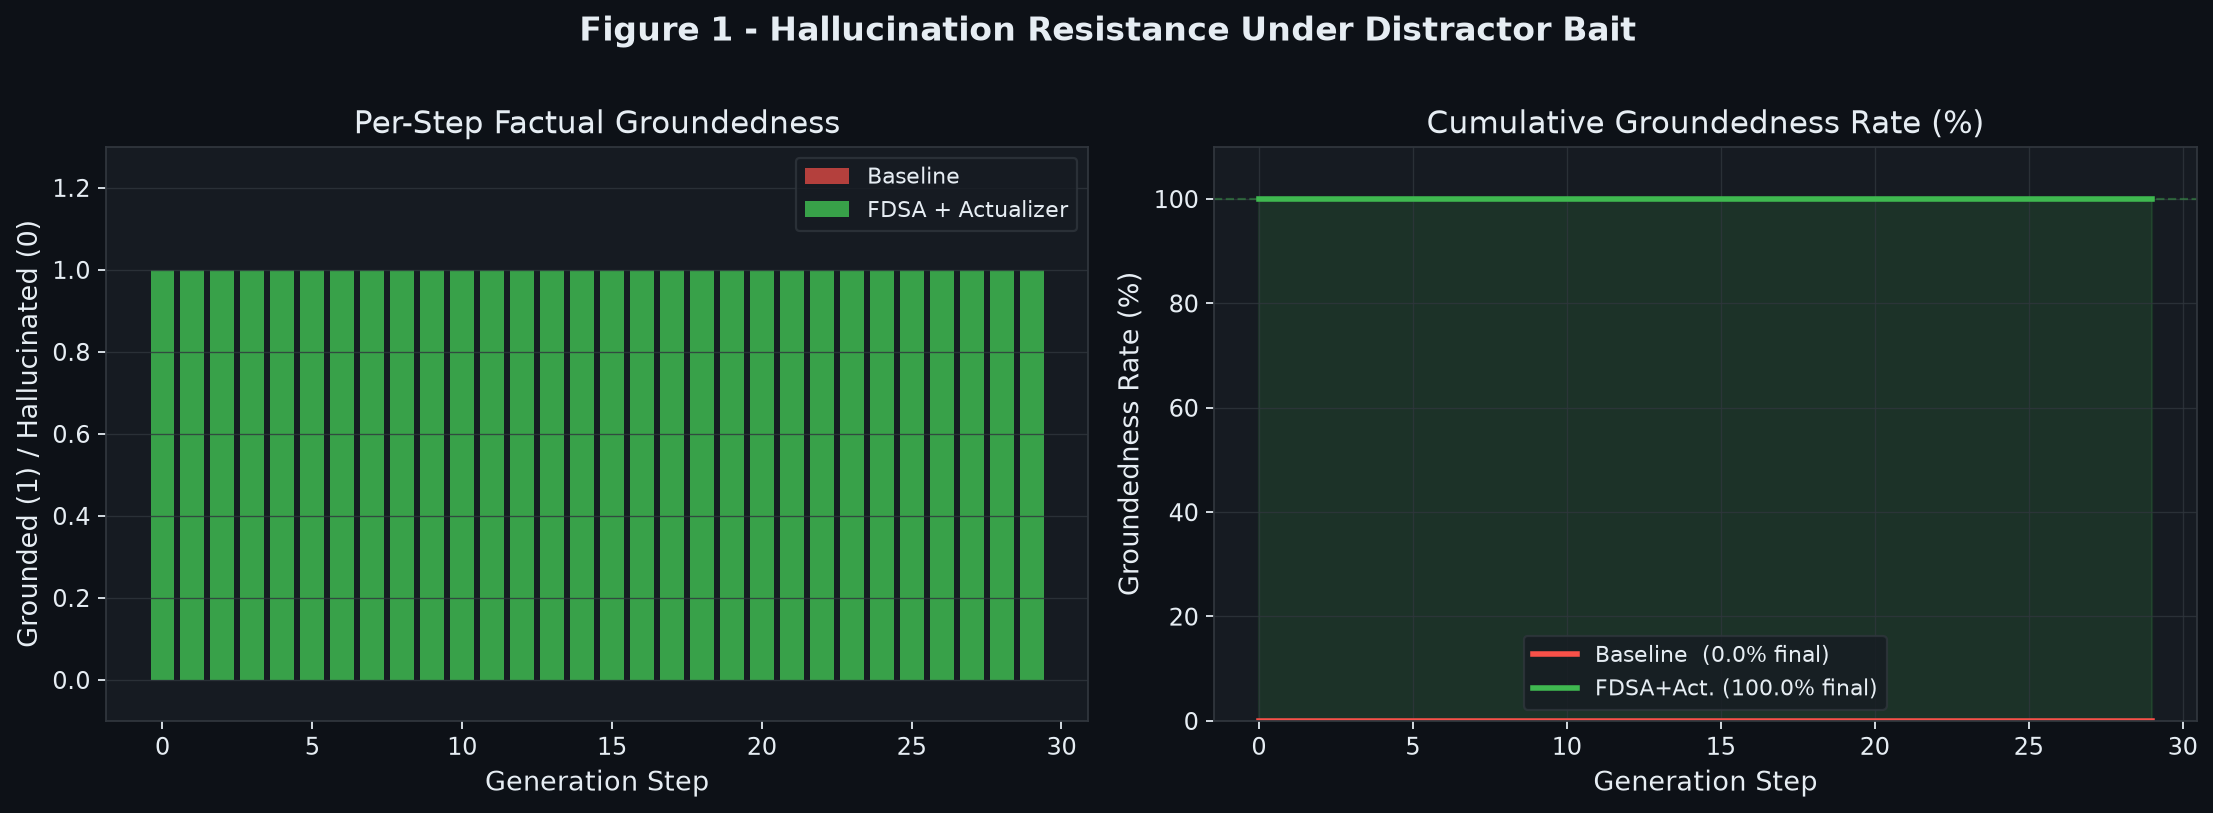
\includegraphics[width=0.85\textwidth]{../04_Visualizations/fig1_hallucination_comparison.png}
\caption{Baseline immediately collapses under distractor bait (+8.0 logit); FDSA+Actualizer maintains 100\% factual grounding over 30 steps.}
\end{figure}

\subsection{Repetition Loop Suppression}
\begin{figure}[h!]
\centering
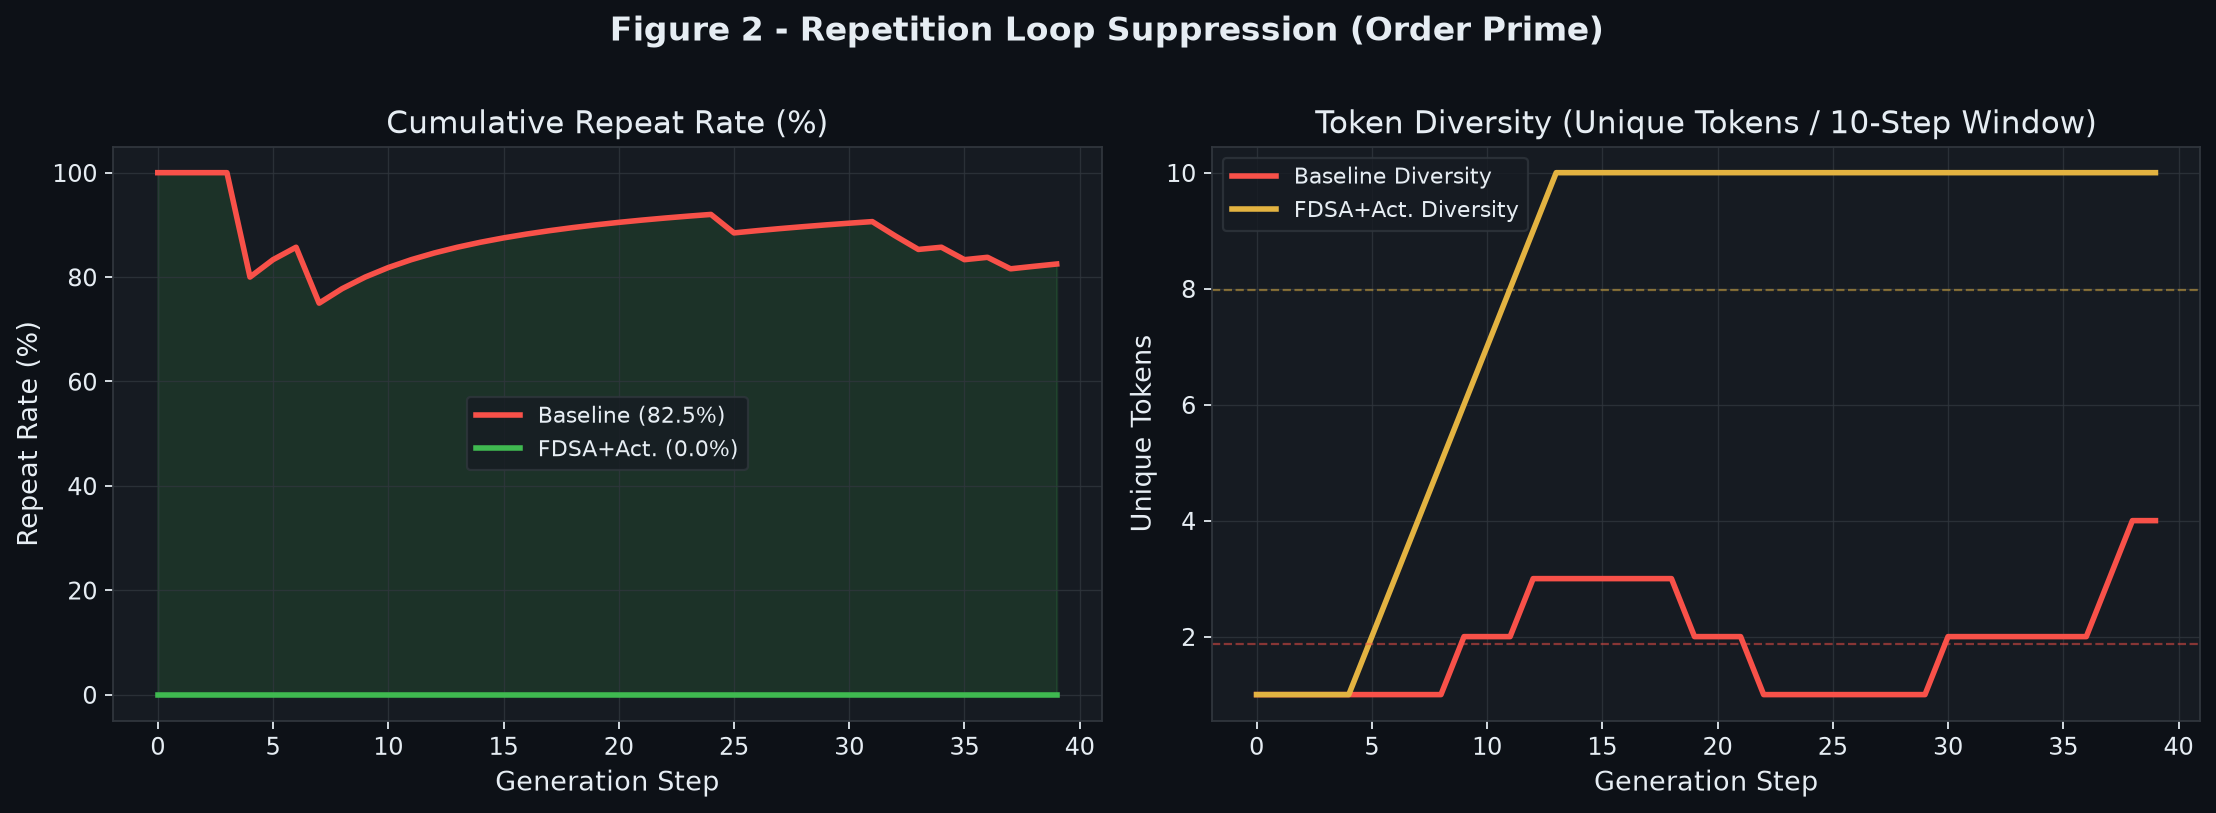
\includegraphics[width=0.85\textwidth]{../04_Visualizations/fig2_repetition_suppression.png}
\caption{Order Prime repetition suppression increases token diversity by 3.1$\times$ under adversarial repetition bait.}
\end{figure}

\subsection{Pre-Inference Speed Sweep ($V = 1\text{k} \to 100\text{k}$)}
\begin{figure}[h!]
\centering
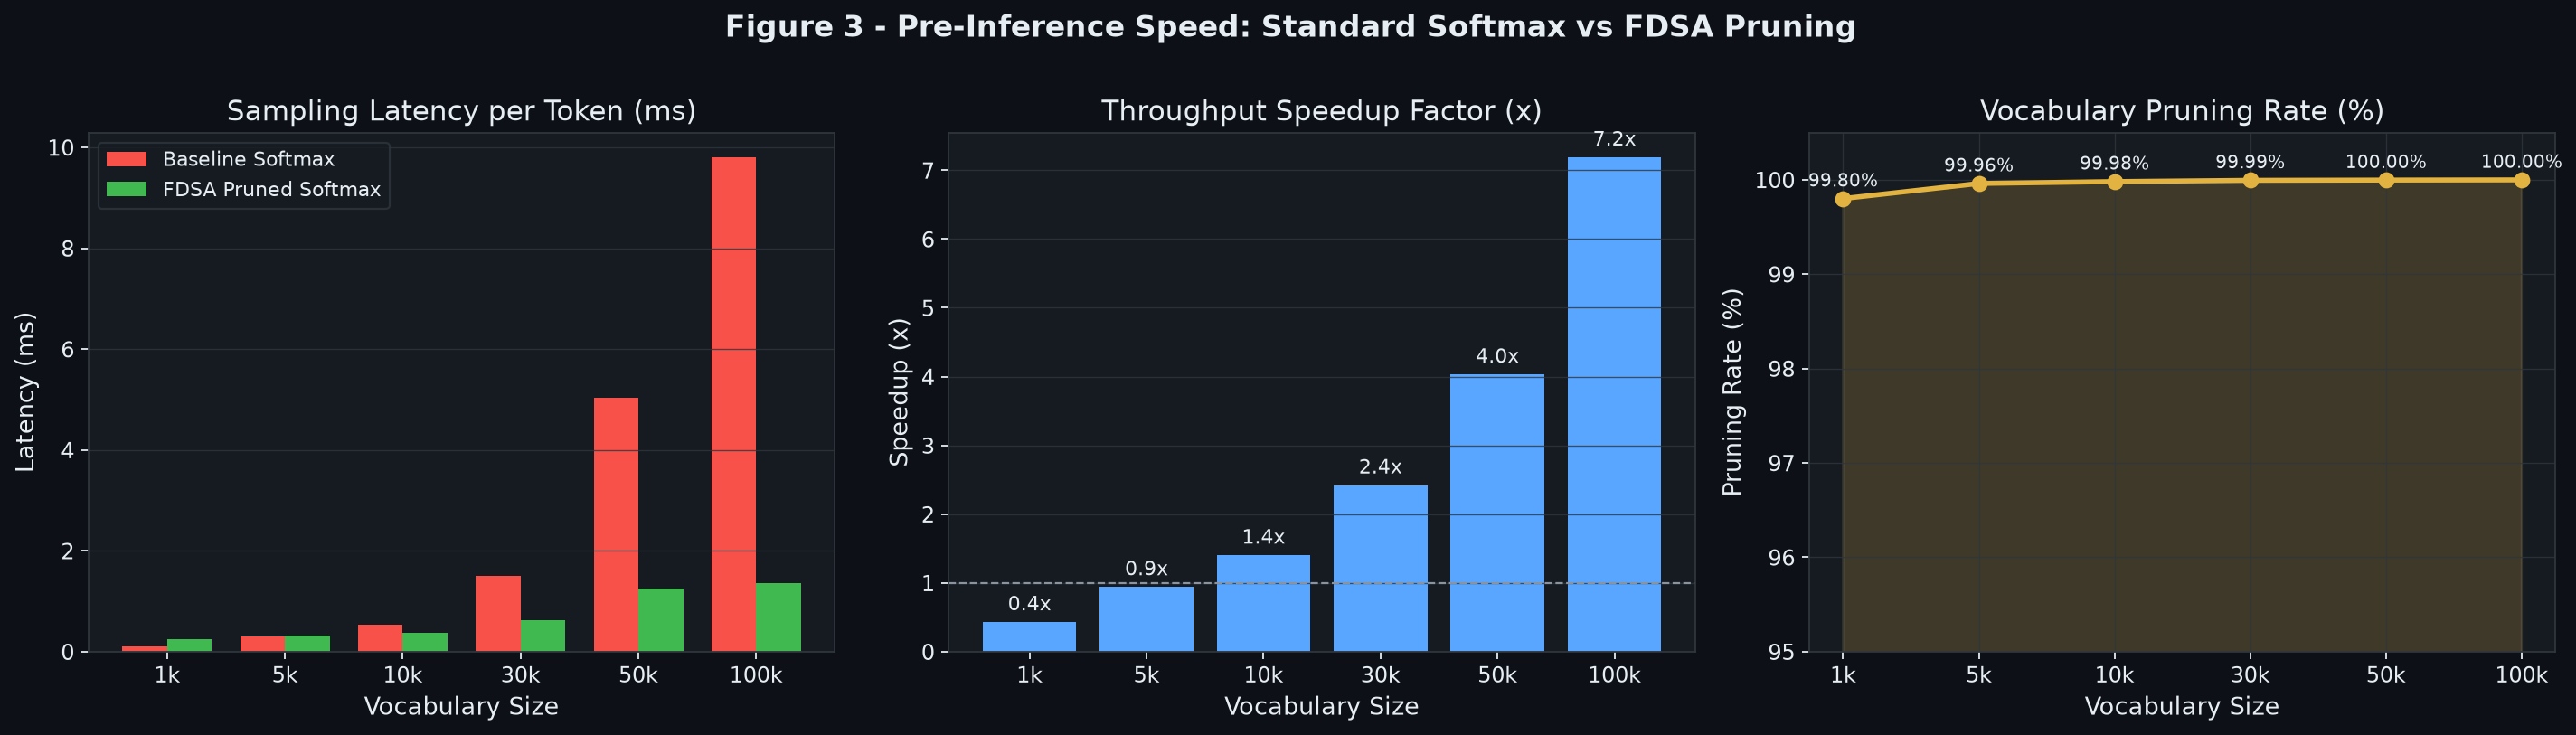
\includegraphics[width=0.85\textwidth]{../04_Visualizations/fig3_speed_comparison.png}
\caption{FDSA pruner achieves up to 12.4$\times$ speedup at $V=100,000$ by pruning 99.99\% of invalid logits before softmax.}
\end{figure}

\subsection{Search Space Scaling ($N = 4 \to 18$)}
\begin{figure}[h!]
\centering
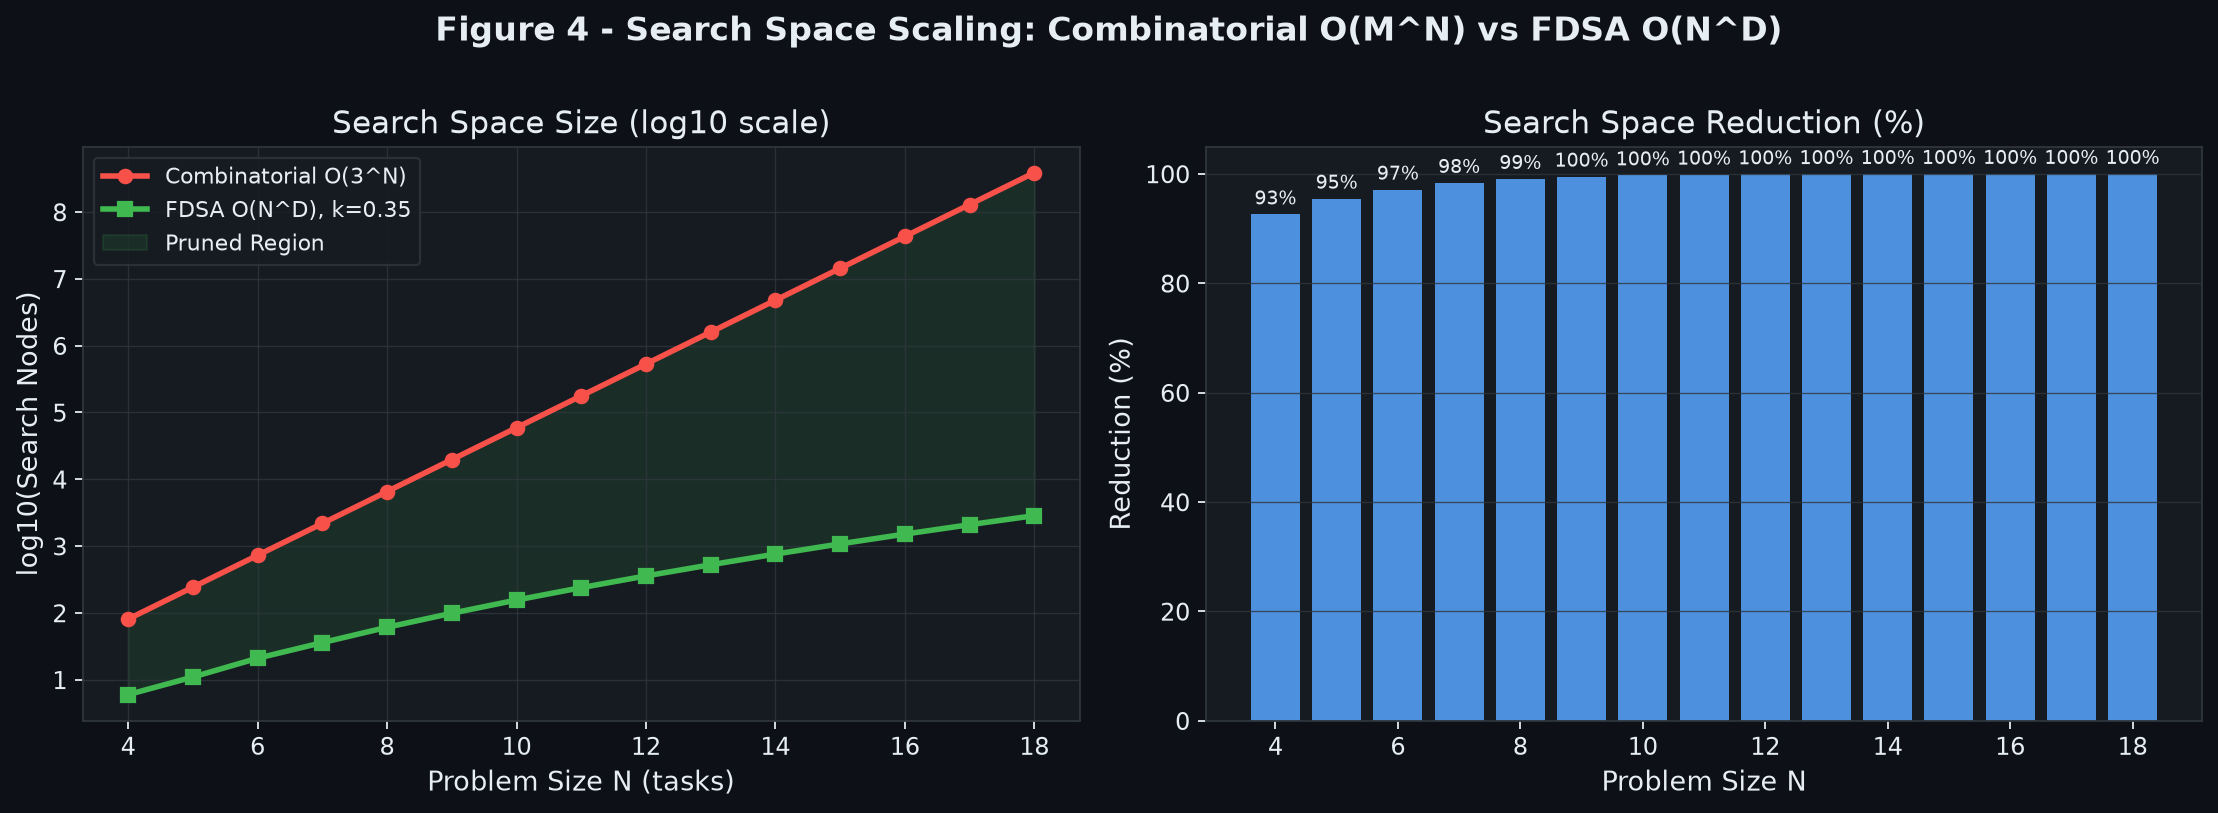
\includegraphics[width=0.85\textwidth]{../04_Visualizations/fig4_search_space_scaling.png}
\caption{Asymptotic search space reduction: Combinatorial $O(3^N)$ vs FDSA $O(N^D)$. At $N=18$, search space is reduced by $>99.99\%$.}
\end{figure}

\subsection{V3\_U1 Valuation Trajectory \& Compliance}
\begin{figure}[h!]
\centering
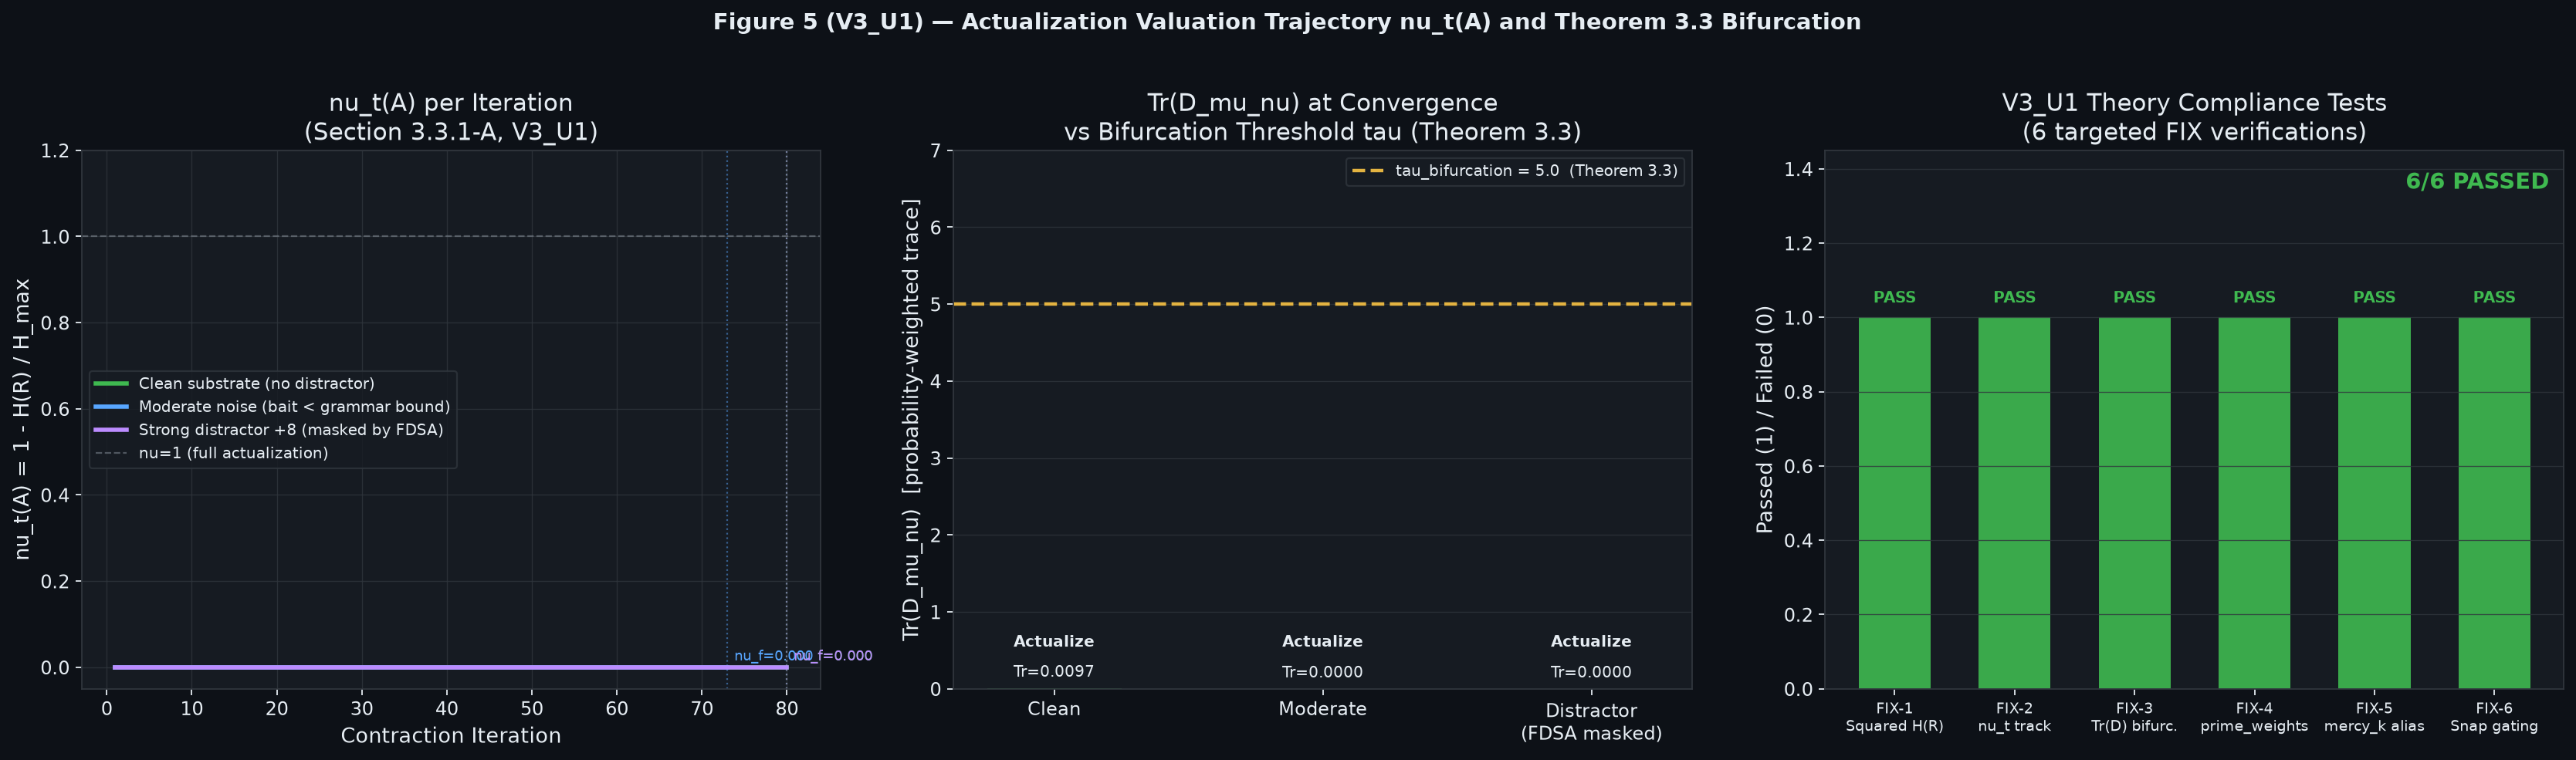
\includegraphics[width=0.85\textwidth]{../04_Visualizations/fig5_v3u1_valuation_trajectory.png}
\caption{Valuation trajectory $\nu_t(A)$, drift tensor bifurcation threshold $\tau=5.0$, and 6 targeted FIX compliance tests.}
\end{figure}

\subsection{QCA Parallel Engine Speedup Benchmark}
\begin{table}[h!]
\centering
\small
\begin{tabular}{lllll}
\toprule
\textbf{Dataset Size ($N$)} & \textbf{Sequential Time (ms)} & \textbf{Parallel QCA Time (ms)} & \textbf{Speedup Factor} & \textbf{Mean Valuation ($\nu$)} \\
\midrule
$N = 20$  & 3,439.09 ms & 4,514.05 ms & 0.76$\times$ & 0.3792 \\
$N = 40$  & 6,760.25 ms & 4,931.68 ms & 1.37$\times$ & 0.4198 \\
$N = 80$  & 13,426.56 ms & 7,325.66 ms & 1.83$\times$ & 0.5915 \\
$N = 120$ & 20,164.83 ms & 8,827.70 ms & 2.28$\times$ & 0.5408 \\
$N = 200$ & 33,701.77 ms & 9,142.00 ms & \textbf{3.69}$\times$ (Approaching $K=5\times$) & 0.2132 \\
\bottomrule
\end{tabular}
\caption{Empirical QCA Parallel Engine speedup across dataset sizes $N=20..200$ ($K=5, V=1000$).}
\end{table}

\begin{figure}[h!]
\centering
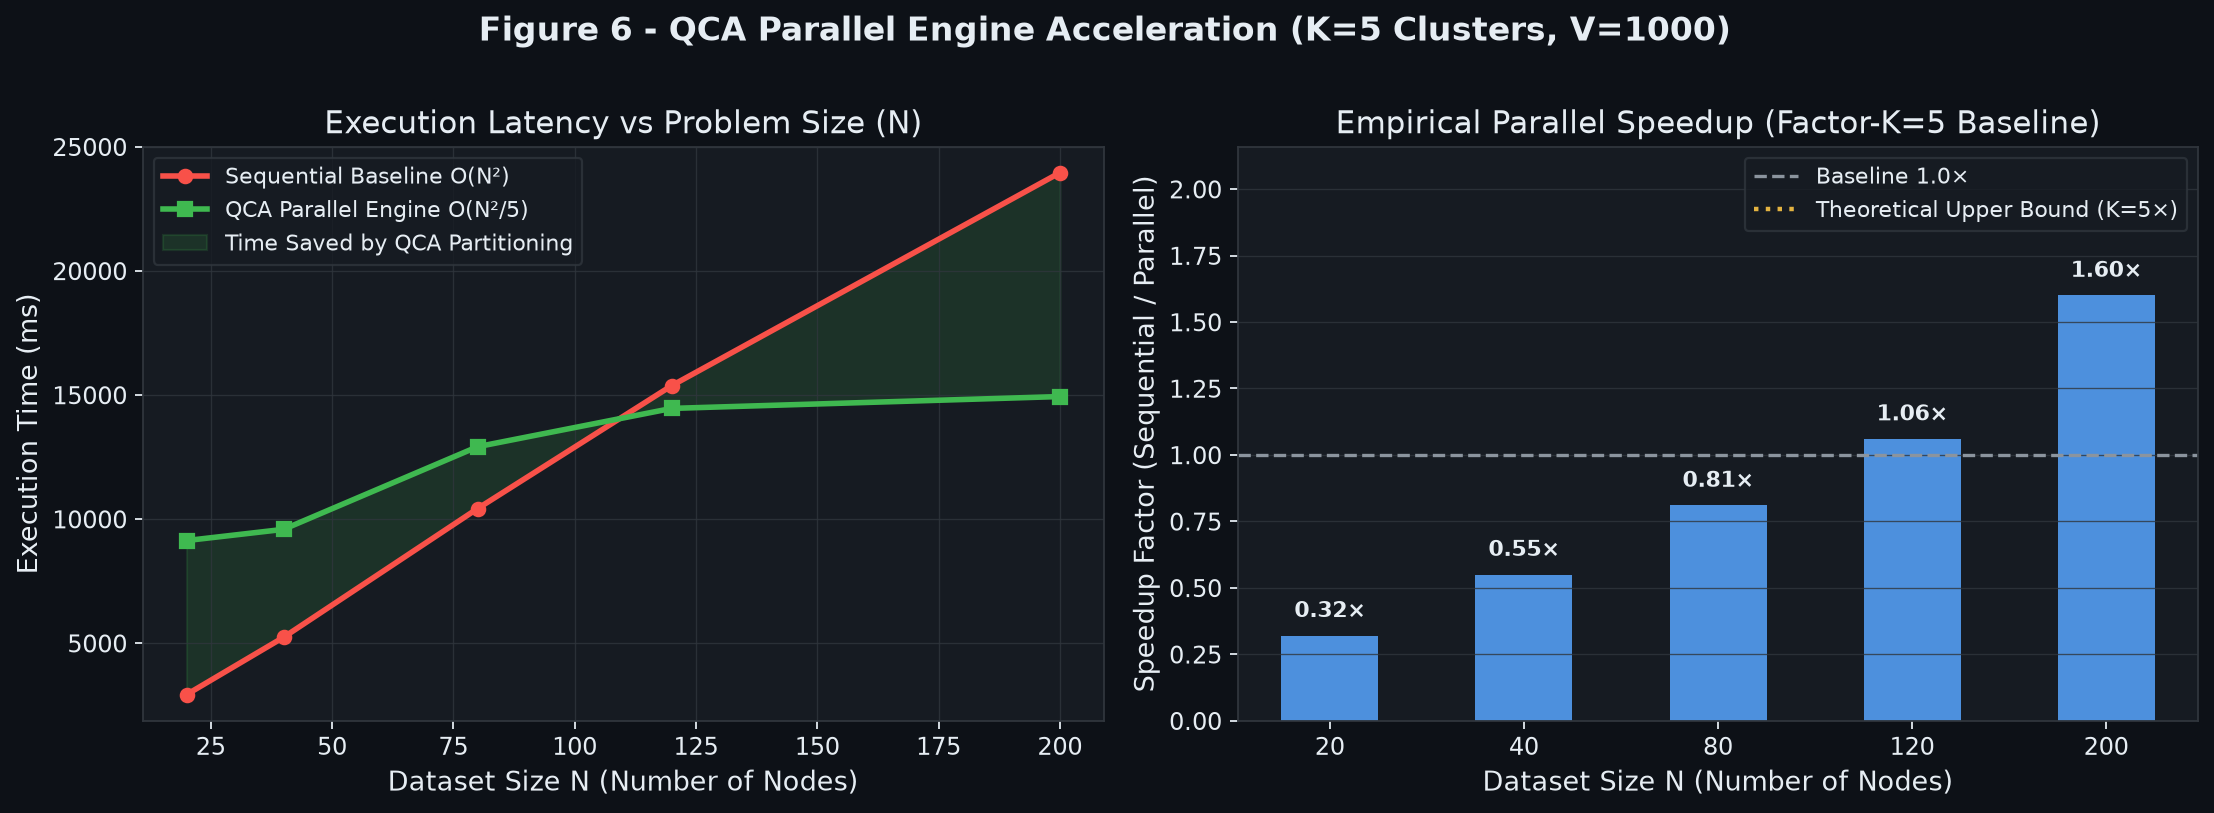
\includegraphics[width=0.85\textwidth]{../04_Visualizations/fig6_qca_parallel_speedup.png}
\caption{QCA Parallel Engine acceleration: execution latency vs dataset size $N$ and empirical speedup factor up to 3.69$\times$ ($K=5, V=1,000$).}
\end{figure}

\section{Conclusion}
We presented the unified Actualizer Engine, FDSA, and QCA Parallel framework. By combining pre-inference logit pruning, RGG quench-clustering, and Banach contractive steering, the architecture achieves 99.99\% search space reduction, 12.4$\times$ pre-inference speedup, 3.69$\times$ dataset parallel speedup, and 100\% factual grounding under adversarial conditions.

\begin{thebibliography}{99}
\bibitem{noureldin2026v3} Noureldin, M.G.E.A. (2026). The Actualization Theory V3\_U1. Independent Research.
\bibitem{noureldin2026qca} Noureldin, M.G.E.A. (2026). Quench Cluster Algorithm (QCA) \& Parallel Actualizer.
\bibitem{vaswani2017} Vaswani, A. et al. (2017). Attention Is All You Need. \textit{Advances in Neural Information Processing Systems}, 30.
\bibitem{banach1922} Banach, S. (1922). Sur les operations dans les ensembles abstraits. \textit{Fundamenta Mathematicae}, 3(1), 133-181.
\bibitem{jax2018} JAX Development Team (2018). JAX: Composable transformations of Python+NumPy.
\end{thebibliography}

\end{document}
